\documentclass{article}
\usepackage{amsmath,amssymb}
\usepackage{fullpage}
\usepackage{enumerate}
\usepackage{tikz}

\newcommand{\dsum}{\displaystyle\sum}
\newcommand{\dint}{\displaystyle\int}
\newcommand{\abs}[1]{\displaystyle\left\lvert#1\right\rvert}
\newcommand{\dbcup}{\displaystyle\bigcup}
\newcommand{\dbcap}{\displaystyle\bigcap}
\newcommand{\dcup}{\displaystyle\cup}
\newcommand{\dcap}{\displaystyle\cap}
\newcommand{\Pb}{\mathbb{P}}
\newcommand{\Eb}{\mathbb{E}}
\newcommand{\soln}[1]{\\ \textbf{Solution}: #1}
\newcommand{\bkt}[1]{\left(#1\right)}
\title{MA2040: Probability, Statistics and Stochastic Processes\\
Problem Set-III}
\author{Sivaram Ambikasaran}
\begin{document}
	\maketitle
	\begin{enumerate}
		\item
		If $X_1,X_2,\ldots,X_n$ are independent random variables having the same probability density function $f_X(x)$, what is the probability density function for the random variable $Y=\text{min}\{X_1,X_2,\ldots,X_n\}$?\\
		\textbf{Solution}: $$P(Y \geq y) = P(X_1 \geq y, X_2 \geq y, \ldots, X_n \geq y) = P(X_1 \geq y)P(X_2 \geq y) \ldots P(X_n \geq y)$$
		Hence, we obtain that
		$$1-F_Y(y) = \bkt{1-F_X(y)}^n$$
		$$f_Y(y) = nf_X(y)\bkt{1-F_X(y)}^{n-1}$$
		\item
		A random variable $X$ has a probability density function as shown below.
		\begin{center}
		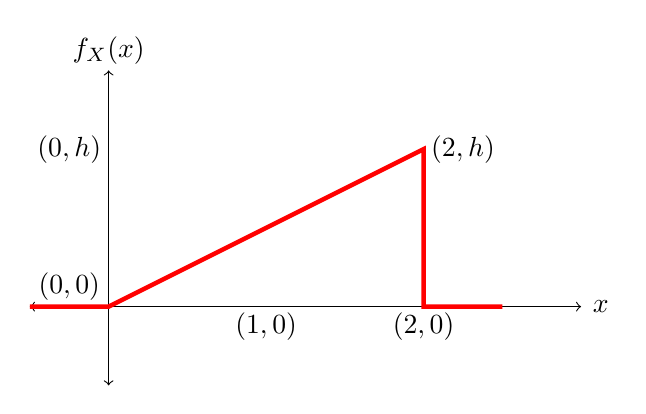
\begin{tikzpicture}[scale=2]
			\draw [<->] (-0.5,0) -- (3,0);
			\draw [<->] (0,-0.5) -- (0,1.5);
			\node at (3.125,0) {$x$};
			\node at (0,1.625) {$f_X(x)$};
			\draw [ultra thick,red] (-0.5,0) -- (0,0) -- (2,1) -- (2,0) -- (2.5,0);
			\node at (-0.25,0.125) {$(0,0)$};
			\node at (1,-0.125) {$(1,0)$};
			\node at (2,-0.125) {$(2,0)$};
			\node at (-0.25,1) {$(0,h)$};
			\node at (2.25,1) {$(2,h)$};
		\end{tikzpicture}
		\end{center}
		\begin{enumerate}
			\item
			Determine $h$
			\soln{Area equals one implies $h=1$}
			\item
			Determine the cumulative distribution function\\
			\soln{
			$F_X(x) =
			\begin{cases}
			0 & \text{if }x \leq 0\\
			x^2/4 & \text{if }x \in [0,2]\\
			1 & \text{if }x \geq 2
			\end{cases}
			$
			}
			\item
			Compute the mean\\
			\soln{
			We have
			$$\Eb\bkt{X} = \dint_0^2 x f_X(x)dx = \dint_0^2 x \cdot \frac{x}2 dx = 4/3$$
			}
			\item
			Compute the variance\\
			\soln{
			$$\Eb\bkt{X^2} = \dint_0^2 x^2 f_X(x)dx = \dint_0^2 x^2 \cdot \frac{x}2 dx = 2 \implies \text{Var}\bkt{X} = 2/9$$
			}
			\item
			Determine the probability that $X \in \bkt{1,2}$.\\
			\soln{
			$$\Pb\bkt{X \in (1,2)} = \dint_1^2 f_X(x)dx = \dint_1^2 x/2 dx = 3/4$$
			}
		\end{enumerate}
		\item
		The median $m$ of a probability density function is defined as the value of $m$ such that
		$$\dint_{-\infty}^m f(x) dx = \dint_m^{\infty} f(x) dx =1/2$$
		Essentially, the median splits the distribution into two equal halves. Prove that the median is the best predictor if one wants to minimize the expected value of the absolute error, i.e., $\mathbb{E}\bkt{\abs{X-c}}$ is minimized when $c$ is the median of the underlying distribution.
		\soln{
		We have
		$$\Eb\bkt{\abs{X-c}} = \dint_{-\infty}^c \bkt{c-x}f_X(x)dx + \dint_c^{\infty} \bkt{x-c}f_X(x)dx$$
		Differentiating with respect to $c$, we obtain
		$$\int_{-\infty}^c f_X(x)dx = \dint_c^{\infty}f_X(x)dx$$
		We also have that
		$$\int_{-\infty}^c f_X(x)dx + \dint_c^{\infty}f_X(x)dx = 1$$
		Hence, this gives us that
		$$\int_{-\infty}^c f_X(x)dx = \dint_c^{\infty}f_X(x)dx = 1/2$$
		}
		\item
		Let $X$ be a random variable, whose pdf is given by
		$$f_X(x) = \begin{cases}
		0 & \text{ if }x \leq 0\\
		xe^{-x^2/2} & \text{ if }x>0
		\end{cases}$$
		Find the pdf for the random variable $Y=X^2$.
		\soln{
		Since $Y=X^2$ is an increasing function on $[0,\infty)$, we have
		$$f_Y(y) = f_X(\sqrt{y}) \dfrac{dx}{dy} = \dfrac{f_X(\sqrt{y})}{2\sqrt{y}} = 1/2e^{-y/2}$$
		}
		\item
		Let $X$ be a uniform random variable on the interval $[0,1]$. Consider the random variable $Y=g\bkt{X}$, where
		$$g(x) = \begin{cases}
		1 & \text{ if }x \leq 1/3\\
		2 & \text{ else}
		\end{cases}$$
		Find the probability mass function of $Y$ and compute its expected value.\\
		\soln{
		$$\Pb\bkt{Y=1} = \Pb\bkt{X \leq 1/3} = 1/3$$
		$$\Pb\bkt{Y=2} = \Pb\bkt{X \geq 1/3} = 2/3$$
		}
		\item
		Show the expected value of a random variable $X$ can also be obtained as
		$$\Eb\bkt{X} = \dint_0^{\infty} \Pb \bkt{X > x}dx - \dint_0^{\infty} \Pb\bkt{X < -x}dx$$
		\soln{
		We have $X = X^+ - X^-$, where $X^+ = \max\{X,0\}$ and $X^- = \max\{-X,0\}$. Note that
		$$X^+ = \dint_0^{\infty} I\bkt{X > t}dt$$
		and
		$$X^- = \dint_{-\infty}^0 I\bkt{X \leq t}dt$$
		where $I$ is the indicator function that takes the value $1$, when the argument is true and takes the value $0$, when the argument is false. We have
		$$\Eb\bkt{X} = \Eb\bkt{X^+-X^-}$$
		which gives us what we want. Note that expectation of the indicator function is nothing but the probability of the argument.
		}
		\item
		A defective coin minting machine produces coins whose probability of heads is a random variable $Y$ with PDF
		$$f_Y\bkt{y} = \begin{cases}
		y \exp\bkt{y} & \text{ if }y \in [0,1]\\
		0 & \text{ otherwise}
		\end{cases}$$
		A coin produced by this machine is selected and tossed repeatedly, with successive tosses assumed independent.
		\begin{enumerate}
			\item
			Find the probability that a coin toss results in head.\\
			$$\dint_0^1 y f_Y(y)dy$$
			\item
			Given that a coin toss resulted in heads, find the conditional PDF of $Y$.\\
			$$ $$
			\item
			Given that the first coin toss resulted in heads, find the conditional probability of heads on the next toss.
		\end{enumerate}
		\item
		Let the random variables $X$ and $Y$ have a joint PDF, which is uniform over the triangles with vertices $(0,0)$, $(0,1)$ and $(1,0)$.
		\begin{enumerate}
			\item
			Find the joint PDF of $X$ and $Y$.\\
			\soln{
			$f_{XY}(x,y) = 2$ over the triangle.
			}
			\item
			Find the marginal PDFs.\\
			\soln{
			$$f_X(x) = \dint_{y=0}^{1-x} 2dy = 2\bkt{1-x}$$
			$$f_Y(y) = \dint_{x=0}^{1-y} 2dx = 2\bkt{1-y}$$			
			}
			\item
			Find the conditional PDFs.\\
			\soln{
			$$f_{X \mid Y=y} = \dfrac1{1-y}$$
			$$f_{Y \mid X=x} = \dfrac1{1-x}$$
			}
		\end{enumerate}
		\item
		Chennai's temperature is modeled as a normal random variable with a mean temperature of $34^{\circ}$C and a standard deviation of $5^{\circ}$C. What is the probability that the temperature at a randomly chosen time will exceed $45^{\circ}$C?\\
		\soln{
		$z = \dfrac{45-34}5 = 2.2$. $\Phi\bkt{2.2} = 0.9861$. Hence, desired probability is $1-0.9861 = 0.1039$.
		}
		\item
		A surface is ruled with parallel lines, which are at a distance $d$ from each other. Suppose that we throw a needle of length $l$ on the surface at random. What is the probability that the needle with intersect one of the lines? (NOTE: You will need to treat the case $d<l$ and $d>l$ separately.)\\
		\soln{
		Page 161. Bertsekas.
		$$d > l: \dfrac{2l}{\pi d}$$
		$$d < l: \dfrac2{\pi} \arccos\bkt{\dfrac{d}l} + \dfrac2{\pi} \dfrac{l}d \bkt{1-\sqrt{1-\bkt{\dfrac{d}l}^2}}$$
		}
		\item
		Consider two continuous random variables $Y$ and $Z$ and a random variable $X$ that is equal to $Y$ with a probability $p$ and equals $Z$ with a probability $1-p$. Obtain the pdf of $X$ interms of the pdf's of $Y$ and $Z$.\\
		\soln{
		$$F_X(x) = \Pb\bkt{X \leq x} = p \Pb\bkt{Y \leq x} + \bkt{1-p} \Pb\bkt{Z \leq x}$$
		Hence,
		$$f_X(x) = p f_Y(x) + \bkt{1-p} f_Z(x)$$
		}
	\end{enumerate}
\end{document}